% Suggested insertion point:
% Place this fragment in the Results section, immediately after the paragraph
% that ends "This regime map is what the equation alone cannot deliver..." and
% immediately before \section{Discussion}.

\subsection{Representative graph and accessibility comparisons}
\label{sec:representative-access}

The headline scenarios in Figures~\ref{fig:headline-networks} and
\ref{fig:ccdf} establish the main comparative statics of the generalized
attachment kernel. To make those regimes more directly comparable to the
transport-growth extensions below, Figure~\ref{fig:headline-access-gallery}
re-expresses the validated headline cases as paired graph realizations and
gravity-accessibility fields. This figure does not introduce a new model
family; rather, it provides a common visual baseline for interpreting the
planarity and accessibility extensions.

Three patterns are especially clear. First, the BA benchmark and the
spatial-only case retain visibly strong hubs, but the spatial-only case
compresses the network geographically and produces a more concentrated local
access field. Second, the capacity-only and general-model cases sharply limit
hub size, which is reflected in flatter accessibility surfaces and lower
realized maximum degree. Third, the combined general model remains the most
transport-like of the four baseline regimes: it preserves the short-link logic
of the spatial-only case while inheriting the bounded hub structure of the
capacity-constrained case. These paired graph/accessibility panels therefore
anchor the later extension figures by showing what the already-validated
baseline families look like before any explicit planarity or
accessibility-weighted extensions are activated.

\begin{figure}[htbp]
\centering
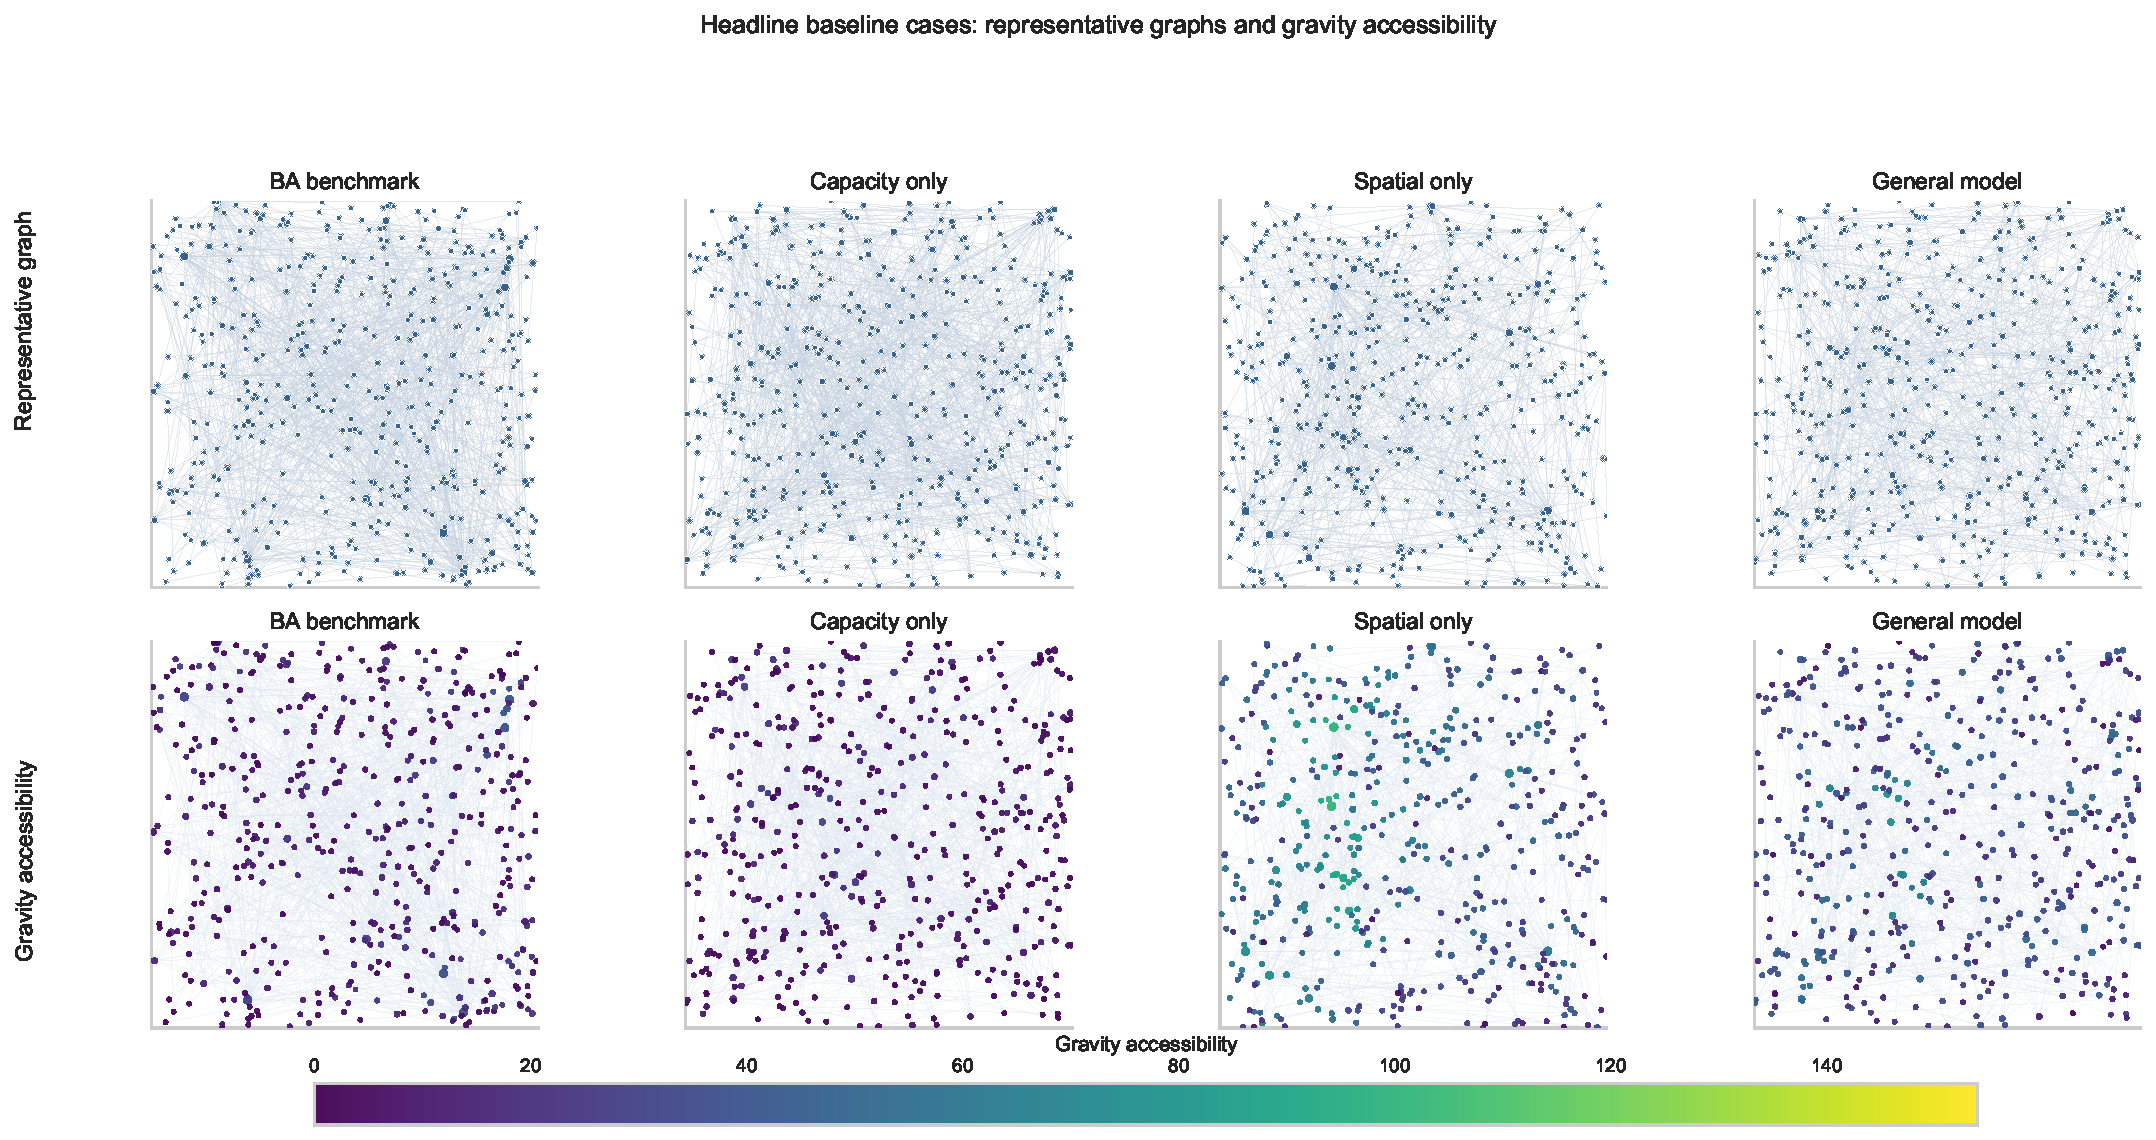
\includegraphics[width=0.98\textwidth]{../results/research_program_20260407_medium/paper_replication/figures/figure_headline_graph_access_gallery.pdf}
\caption{Representative baseline regimes shown as paired graph realizations
and gravity-accessibility fields. The top row shows one representative
realization for each headline scenario from the validated medium replication
bundle; the bottom row colors the same realized nodes by gravity
accessibility on a common scale. The figure provides a direct comparator for
the extension results below by showing how the BA benchmark, capacity-only,
spatial-only, and full generalized model differ not only in morphology but
also in their induced accessibility fields.}
\label{fig:headline-access-gallery}
\end{figure}

\subsection{Transport-growth extensions: planarity and accessibility}
\label{sec:extensions}

The replication results above establish that the generalized attachment kernel
recovers the intended headline comparative statics. A natural next question is
whether the exploratory transport-oriented extensions merely decorate those
baseline regimes or instead define substantively new growth families. We
therefore ran a focused extension program centered on two research questions:
\begin{enumerate}[leftmargin=1.5em]
    \item \textbf{RQ1:} Does planarity handling create a genuinely distinct
    growth mechanism, or does it simply constrain the same underlying
    attachment process?
    \item \textbf{RQ2:} Once planarity is active, do alternative accessibility
    semantics (\emph{network}, \emph{seed-only}, and \emph{opportunity})
    produce meaningfully different transport-growth regimes?
\end{enumerate}

These questions imply two testable hypotheses. \textbf{H1} is that
\texttt{split\_crossings} should not behave like a cosmetic rendering of planar
growth; rather, it should create a junction-forming process distinct from both
unconstrained growth and \texttt{reject\_crossings}. \textbf{H2} is that
accessibility semantics should matter most when a split-planarity mechanism is
already active, because they then govern which destinations the emerging
junction-forming process reinforces.

\subsubsection{Results for RQ1: planarity is a mechanism, not just a constraint}

Figure~\ref{fig:extension-planarity} shows that the three planarity rules
generate qualitatively different regimes under otherwise matched conditions.
The unconstrained case remains crossing-rich, with average clustering $0.123$,
mean edge length $0.537$, and about $357$ admitted crossing candidates. The
\texttt{reject\_crossings} regime suppresses crossing admissions entirely and
concentrates growth into a highly triadic planar fabric: clustering rises to
$0.776$ while mean edge length falls to $0.266$. The
\texttt{split\_crossings} regime behaves differently again. It admits local
crossing candidates (about $368$ on average), produces about $93$ split
events, and generates roughly $17{,}626$ intersection nodes, while maintaining
moderate clustering ($0.170$). The mean realized edge length falls to
$0.0046$, not because the network becomes trivial, but because each admitted
crossing is resolved into many short junction-to-junction segments.

The substantive implication is that split-based planarization does not merely
remove crossings after the fact. It changes the node-creation mechanism itself.
The unconstrained case grows by admitting long crossing links, the reject case
grows by forbidding those links and forcing local closure, and the split case
grows by converting admissible crossings into new junctions. These are
different transport-growth processes rather than different renderings of the
same graph.

\begin{figure}[htbp]
\centering
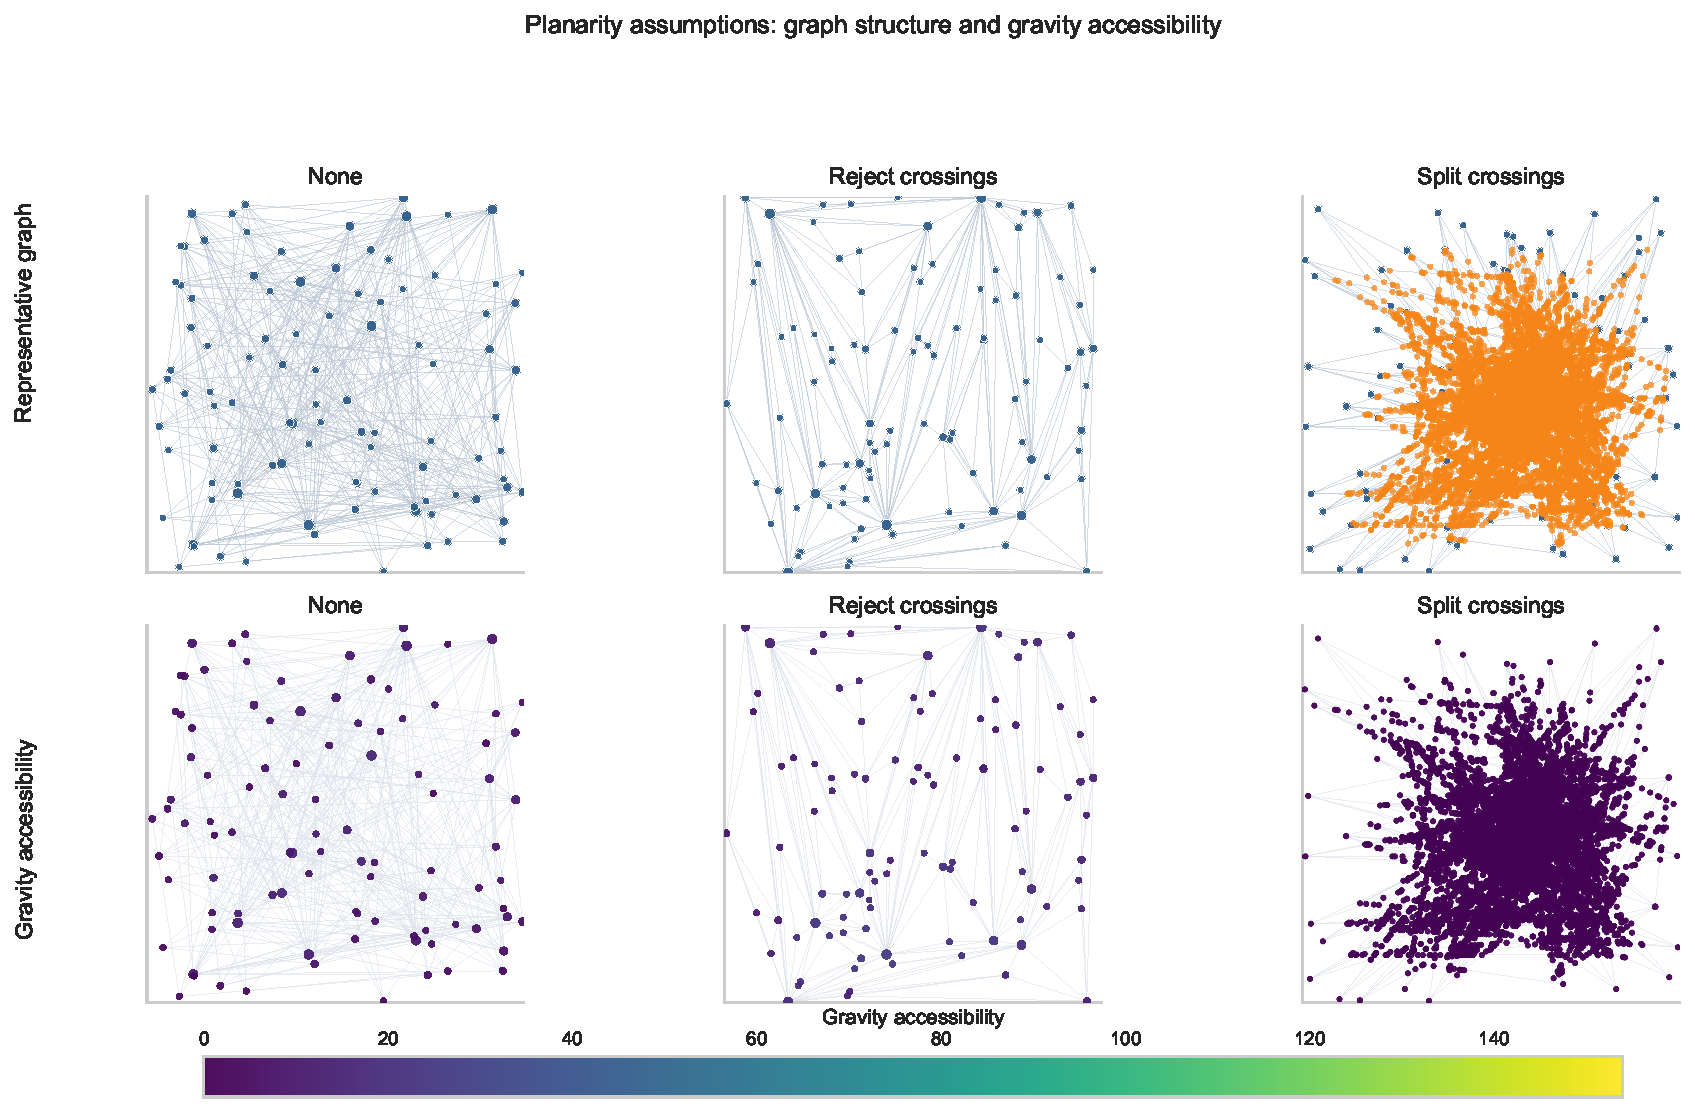
\includegraphics[width=0.98\textwidth]{../results/beyond_paper_focused_20260422_medium/figures/figure_extension_planarity_gallery.pdf}
\caption{Representative planarity-extension realizations and their gravity
accessibility fields, shown on the same accessibility scale used in
Figure~\ref{fig:headline-access-gallery}. The top row shows one representative
graph for each planarity rule under matched free-geometry conditions. The
bottom row colors the same realized nodes by gravity accessibility.
Unconstrained growth remains crossing-rich, \texttt{reject\_crossings}
concentrates growth into a highly triadic planar fabric, and
\texttt{split\_crossings} produces a dense junction-forming regime with many
generated intersection nodes. The figure therefore illustrates visually that
the three planarity rules define different transport-growth mechanisms rather
than alternative renderings of the same graph.}
\label{fig:extension-planarity}
\end{figure}

\subsubsection{Results for RQ2: accessibility semantics matter within split-planar growth}

Figure~\ref{fig:extension-access} shows the second extension result. Under a
shared split-capable transport-growth design, the split machinery remains
active across all three split cases, but the meaning of accessibility changes
the realized access field dramatically. The split case with target-only
\emph{network} accessibility produces the highest mean gravity access
($121.56$) and cumulative access ($352.23$). When both arrivals and target
selection are governed by \emph{opportunity} access, the resulting access field
is lower but still substantial (gravity access $60.99$, cumulative access
$177.29$). When both arrivals and targets use \emph{seed-only} access, mean
gravity access falls to $3.49$ and mean cumulative access to $8.98$.

What is important here is not only that the values differ, but that they differ
while the split machinery remains active at comparable intensity. The three
split cases all admit roughly $172$ crossing candidates and produce about
$168$--$169$ split events, yet their realized accessibility fields are sharply
different. Hence the accessibility semantics are not merely diagnostic labels.
They govern which destinations matter within an otherwise common
junction-forming growth mechanism. In this sense, the accessibility layer
becomes theoretically substantive only once the model includes a transport-like
planarization process capable of generating new junctions.

\begin{figure}[htbp]
\centering
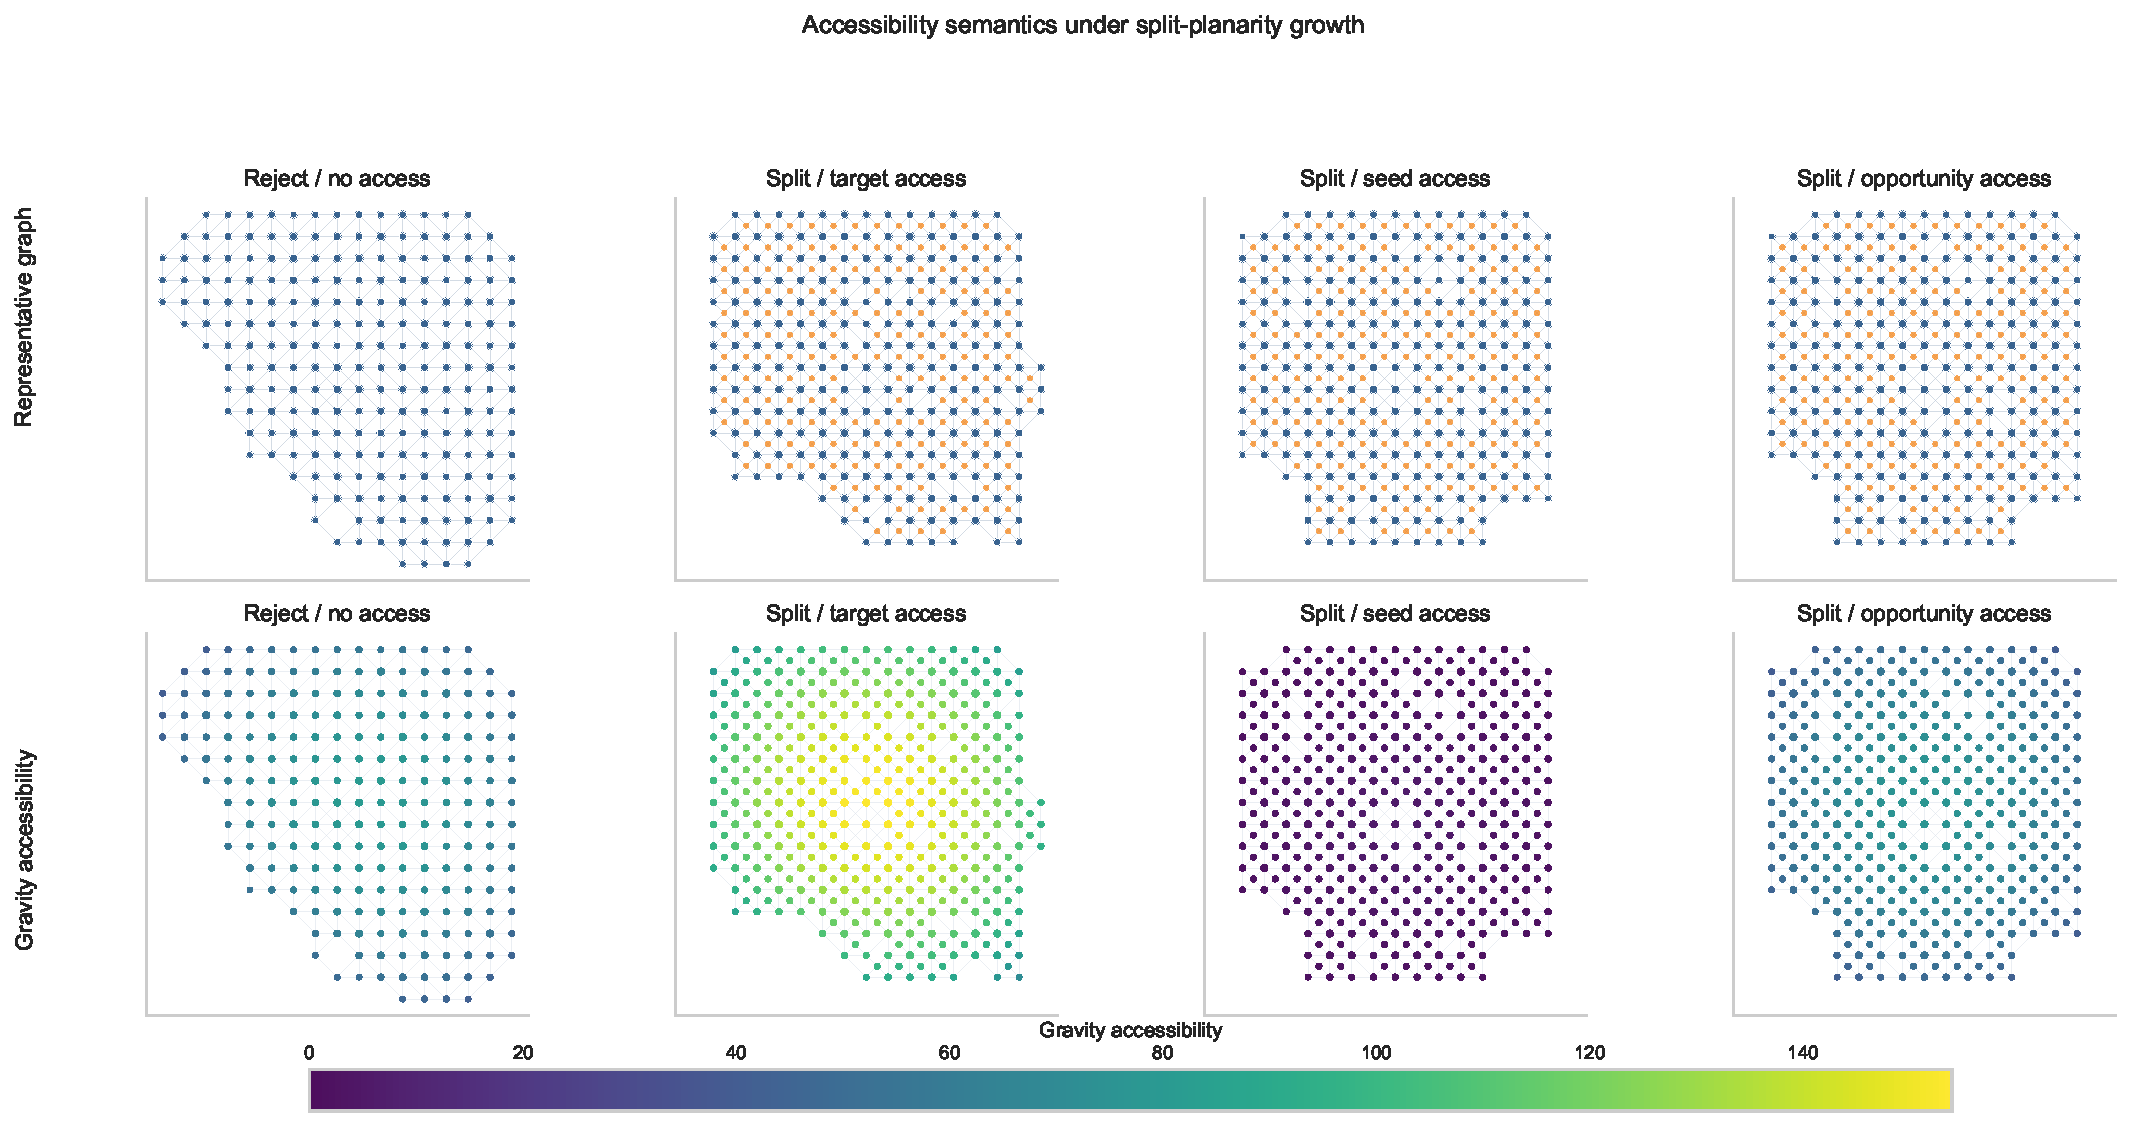
\includegraphics[width=0.98\textwidth]{../results/beyond_paper_focused_20260422_medium/figures/figure_extension_access_gallery.pdf}
\caption{Representative graphs and gravity-accessibility maps for alternative
accessibility semantics under an active split-planarity regime, again using the
same gravity-accessibility scale as the baseline comparison in
Figure~\ref{fig:headline-access-gallery}. The top row shows one representative
graph for each case; the bottom row colors the same realized nodes by gravity
accessibility. Once split-based planarization is active, the chosen
accessibility semantics materially alter the realized accessibility field:
network-based access produces the strongest accessibility regime,
opportunity-based access an intermediate regime, and seed-only access the
weakest. The split mechanism remains active across the split cases, so the
semantics operate by changing which destinations matter rather than by turning
splitting on or off.}
\label{fig:extension-access}
\end{figure}

\subsubsection{Implications for the generalized model}

These extension results suggest that two ideas are worth carrying beyond the
baseline replication exercise. First, split-based planarization can be
interpreted as a junction-forming transport-growth mechanism rather than merely
as a topological constraint. Second, accessibility semantics become
theoretically substantive once such a mechanism is active, because they define
competing destination logics within the same geometric growth process.

This does not mean that the present paper must be rewritten around the
extensions. The baseline generalized model remains the core contribution. But
the focused extension results show that the framework can support a broader
transport-growth interpretation in which planarity shapes how junctions emerge
while accessibility determines which parts of the evolving network become
reinforced.
